\small
% \footnotesize
\centering
\newcommand\irad{4.0cm}
% \newcommand\orad{6cm}
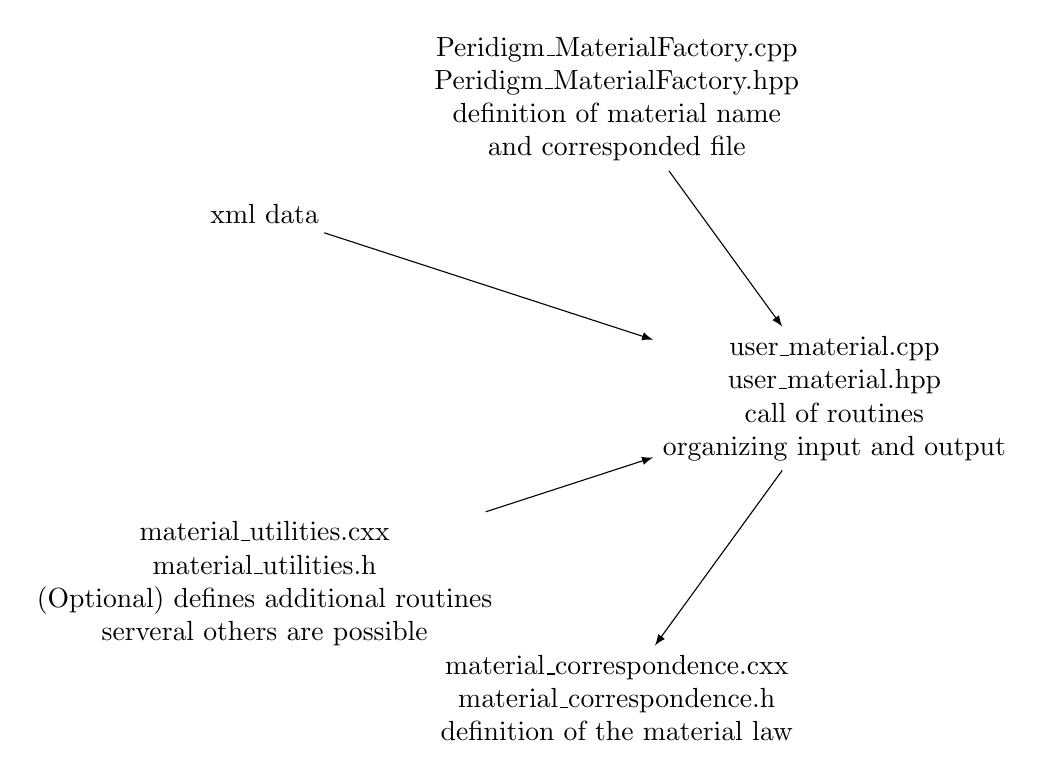
\begin{tikzpicture}

% Variablen
\def\numNodeOnCircle{5}

% Tools
\draw (0:\irad) node[align=center] (Material) {user\_material.cpp\\
user\_material.hpp\\call of routines\\organizing input and output};
\draw (1*360/\numNodeOnCircle:\irad) node[align=center] (PeridigmMaterialFactoryCPP) {Peridigm\_MaterialFactory.cpp\\Peridigm\_MaterialFactory.hpp\\definition of material name  \\and corresponded file};
\draw (2*360/\numNodeOnCircle:\irad) node[align=center] (xml) {xml data};
\draw (3*360/\numNodeOnCircle:\irad) node[align=center] (Routines)    {material\_utilities.cxx\\material\_utilities.h\\(Optional) defines additional routines\\serveral others are possible};
\draw (4*360/\numNodeOnCircle:\irad) node[align=center] (UMAT) {material\_correspondence.cxx\\material\_correspondence.h\\definition of the material law};

% Striche
\draw[-latex] (Material) -- (UMAT);
\draw[-latex] (Routines) -- (Material);
\draw[-latex] (PeridigmMaterialFactoryCPP) -- (Material);
\draw[-latex] (xml) -- (Material);

\end{tikzpicture}

